\documentclass[a4paper,12pt]{article}
\setlength{\oddsidemargin}{-0.33in}
\setlength{\evensidemargin}{0in}
\setlength{\textwidth}{7in}
\setlength{\textheight}{10.2in}
\setlength{\footskip}{.5in}

\setlength{\voffset}{-.5in}
\setlength{\topmargin}{-0.5in}
\setlength{\headheight}{.5in}
\setlength{\headsep}{12pt}

\setlength\parindent{0pt}

% \usepackage{savetrees}
\usepackage{stmaryrd}
\usepackage{hyperref}
\usepackage{color}
\usepackage{outlines}
\usepackage{rotating}
\usepackage{overpic}
\usepackage{algorithm}
\usepackage{algorithmic}
\usepackage{amsmath}
\usepackage{amssymb}
\usepackage{fancyhdr,lastpage}
\usepackage{enumerate}
\usepackage{graphicx}
\usepackage{epstopdf}
\usepackage{rotating}
\usepackage{mathrsfs}
\usepackage{tipa}
\usepackage{setspace}
\usepackage{natbib}

%\doublespacing
\newcommand{\bs}[1]{\boldsymbol{#1}}
\newcommand{\real}[1]{\Re\left\{#1\right\}}
\newcommand{\TD}[2]{\frac{D#1}{D#2}}
\newcommand{\td}[2]{\frac{d#1}{d #2}}
\newcommand{\pd}[2]{\frac{\partial #1}{\partial #2}}
\newcommand{\pdd}[3]{\frac{\partial^2 #1}{\partial #2 \partial #3}}
\newcommand{\pdt}[2]{\frac{\partial^2 #1}{\partial #2 ^2}}
\newcommand{\expv}[1]{\left \langle #1 \right \rangle}
\newcommand{\tensort}[1]{\underline{\underline{#1}}}
\newcommand{\erf}[1]{\mbox{erf}{\left( {#1}\right)}}
\newcommand{\erfc}[1]{\mbox{erfc}{\left( {#1}\right)}}
\newcommand{\ands}{ \ \ \ \mbox{ and } \ \ \ }
\newcommand{\spword}[1]{ \ \ \ \mbox{ {#1} } \ \ \ }

\begin{document}
\title{Polythermal Equation Notes}
\author{Toby Harvey}
\maketitle
\vspace{-1cm}

\section{Map}

The model in \cite{schoof_2016} comes a long history of polythermal models. These notes are an attempt at understand \cite{schoof_2016}, and the background to get there. 

\section{Derivation of Jump conditions}

\subsection{Greve, Hutter, and Spencer continuum mechanics}

Begining with the eulerian description of the balance equation. Eulerian:

\begin{align}
\frac{d}{dt} \int_{B_t} \psi dv = \oint_{\partial B_t} \phi_i^\psi da_i + \int_{B_t} \pi^\psi + \sigma^\psi dv \label{eq:eulerian}
\end{align}

Where $\psi$ is the field quantity in the volume $B_t$ at time $t$, $\phi_i^\psi$ is the flux in the $i$ direction through the boundary $\partial B_t$ at time $t$, with infintesimal area vector $da$. $\pi^\psi$ is the production term, in our case melting or freezing. $\sigma^\psi$ is the supply, which would be external water. First we do the derivation of the local description without jump conditions, which involes moving the total derivative inside the integral of the LHS, and changing the boundary integral to a volume integral in the first term on the RHS. First transforming the LHS of \eqref{eq:eulerian}:

\begin{align}
\frac{d}{dt} \int_{B_t} \psi dv = \int_{B_t} \dot{\psi} dv + \int_{B_t} \psi d\dot{v} \label{eq:balance_lhs}
\end{align}

To transform the second integral on the RHS of the above equation into something useful we need to transform to a lagragian frame of reference and then find the total derivative of the jacobian as follows. First decomposing the volume element into the product of the line elements $dx^{(l)}$:

\begin{align*}
  dv = |e_{ijk} dx_i^{(1)}dx_j^{(2)}dx_k^{(3)}|
\end{align*}
  
If we now consider a line increment of a volume element $dx^{(l)}$ in an eulerian frame it is related to the lagrangian frame of reference using the deformation gradient tensor (\url{https://www.youtube.com/watch?v=rt4wlXOD5S8}, \textcolor{red}{TODO write this out}):

\begin{align}
  dx_i = F_{iA}dX_A, ~~~ F = \pd{x_i}{X_A}
\end{align}

These two relations combine to give us:

\begin{align}
  dv = |e_{ijk}F_{iA}F_{jB}F_{kC}dX^1_AdX^2_BdX^3_C| = |\det(F)||e_{ABC} dX_A^{(1)}dX_B^{(2)}dX_C^{(3)} = |\det(F)|dV = JdV
\end{align}

Now if we take the time derivatve of $dv$ we see that it only goes over the jacobian, because $dV$ is constant since it is in the reference frame:

\begin{align}
d\dot{v} = \dot{J} dV
\end{align}

Here and below the dot denotes the total derivative. Now, the time derivative of the jacobian can be transformed with the following:

\begin{align*}
  &\dot{J} = \frac{d}{dt} \det{(F)} = & (\text{Jacobi's formula})\\
  &J \text{ tr}\left(F^{-1}\frac{dF}{dt}\right)= J \text{ tr}\left(F^{-1}\pd{}{X}\left(\frac{dx}{dt}\right)\right)= J \text{ tr}\left(F^{-1}\pd{u}{X}\right) =  & (\text{chain rule})\\
  &J \text{ tr}\left(F^{-1}\pd{u}{x}\pd{x}{X}\right) = J \text{ tr}\left(F^{-1}\pd{u}{x}F\right) = J \text{ tr}\left(\pd{u}{x}F^{-1}F\right) = \\
  & J \text{ tr}\left(\pd{u}{x}\right) = J (\nabla \cdot u)
\end{align*}

where $u = \pd{x}{t}$ is the velocity. This then plugged in gives:

\begin{align}
  d\dot{v} = \dot{J}dV = (\nabla \cdot u) J dV = u_{i,i} dv
\end{align}

Altogether the LHS of the balance equation \eqref{eq:balance_lhs}, with the total derivative chain ruled out becomes:

\begin{align}
  &\frac{d}{dt} \int_{B_t} \psi dv = \int_{B_t} \dot{\psi} dv + \int_{B_t} \psi d\dot{v} =\\
  &\int_{B_t} \pd{\psi}{t}dv + \int_{B_t}\psi_{,i}u_i dv + \int_{B_t} \psi u_{i,i} dv = \\
  &\int_{B_t} \pd{\psi}{t}dv + \int_{B_t}(\psi u_i)_{i} dv \label{eq:transport-theorem}
\end{align}

Now looking at the first term of the RHS of \eqref{eq:eulerian}, this can be turned to a volume integral with the divergence theorem so:

\begin{align}
\oint_{\partial B_t} \phi_i^\psi da_i = \int_{B_t} \phi_{i,i}^\psi dv
\end{align}

So accounting for all of the terms again in the balance equation gives:

\begin{align}
  &\int_{B_t} \pd{\psi}{t}dv + \int_{B_t}(\psi u_i)_{i} dv = \int_{B_t} \phi_{i,i}^\psi dv + \int_{B_t} \pi^\psi + \sigma^\psi dv =\\
  &\pd{\psi}{t} + (\psi u_i)_{i} = \phi_{i,i}^\psi + \pi^\psi + \sigma^\psi
\end{align}

Now if there is a surface in the volume where this is a finite jump in the same transformations can't be applied because the lack of differentiability, but if we split the total derivative integral on two different sides we get:

\begin{align*}
  &\frac{d}{dt} \int_{B_t} \psi dv = \frac{d}{dt} \int_{B_t} \psi^+ dv + \frac{d}{dt} \int_{B_t} \psi^- dv = ~~~ (\text{by the above derivation})\\
  &\int_{B_t} \pd{\psi^+}{t}dv + \int_{B_t}(\psi^+ u_i)_{i} dv +  \int_{B_t} \pd{\psi^-}{t}dv + \int_{B_t}(\psi^- u_i)_{i} dv = ~~~ (\text{divergance theorem})
 \\
  &\int_{B_t} \pd{\psi^+}{t}dv + \int_{\partial B_t}\psi^+ u_i da_i +  \int_{B_t} \pd{\psi^-}{t}dv + \int_{\partial B_t}\psi^- u_i da_i = ~~~ (\text{splitting the boundary so interface is }l)\\
  &\int_{B_t} \pd{\psi^+}{t}dv + \int_{\partial B_t}\psi^+ u_i da_i - \int_{l}\psi^+ v_i da_i +  \int_{B_t} \pd{\psi^-}{t}dv + \int_{\partial B_t}\psi^- u_i dv + \int_{l}\psi^- v_i da_i =\\
  &\int_{B_t} \pd{\psi}{t}dv + \int_{\partial B_t}\psi u_i da_i - \int_{l}\llbracket\psi v_i\rrbracket da_i
\end{align*}

All together in the balance equation this becomes:

\begin{align}
  \int_{B_t} \pd{\psi}{t}dv + \int_{\partial B_t}\psi u_i da_i - \int_{l}\llbracket\psi v_i\rrbracket da_i = \oint_{\partial B_t} \phi_i^\psi da_i + \int_{B_t} \pi^\psi + \sigma^\psi dv
\end{align}

Now choosing the "pill box" around the interface as the area of integration and reducing it to 0 so that the volume integrals disappear, and surface integrals become:

\begin{align}
  \int_{\partial B_t}\psi u_i da_i = \int_{l}\llbracket \psi u_i \rrbracket da_i, ~~~ \oint_{\partial B_t} \phi_i^\psi da_i = \int_{l} \llbracket \phi_i^\psi \rrbracket da_i
\end{align}


So that:

\begin{align}
  &\int_{l}\llbracket\psi u_i\rrbracket da_i - \int_{l}\llbracket\psi v_i\rrbracket da_i = \int_{l} \llbracket\phi_i^\psi\rrbracket da_i\\
  &\llbracket\psi u_in_i\rrbracket - \llbracket\psi v_in_i\rrbracket = \llbracket\phi_i^\psi n_i\rrbracket\\
  & (\psi u_in_i)^+ - (\psi u_in_i)^- - (\psi v_in_i)^+ + (\psi v_in_i)^- = (\phi_i^\psi n_i)^+ - (\phi_i^\psi n_i)^- \\
  &\llbracket \psi (v_i - u_i)n_i \rrbracket = \llbracket \phi_i^\psi n_i \rrbracket
\end{align}

For which any of the conservation laws can be applied.

\subsection{More intuative derivation}
\subsubsection{Mass conservation}

Considering the small sheet where two seperate fluids meet and mix, we can drive the height of this sheet to zero to get the interface conditions, but first we need to write the conservation laws in integral form including the moving interfaces. This is done by using Reynolds transport theorem which is \eqref{eq:transport-theorem}, but with the divergence theorem used giving:

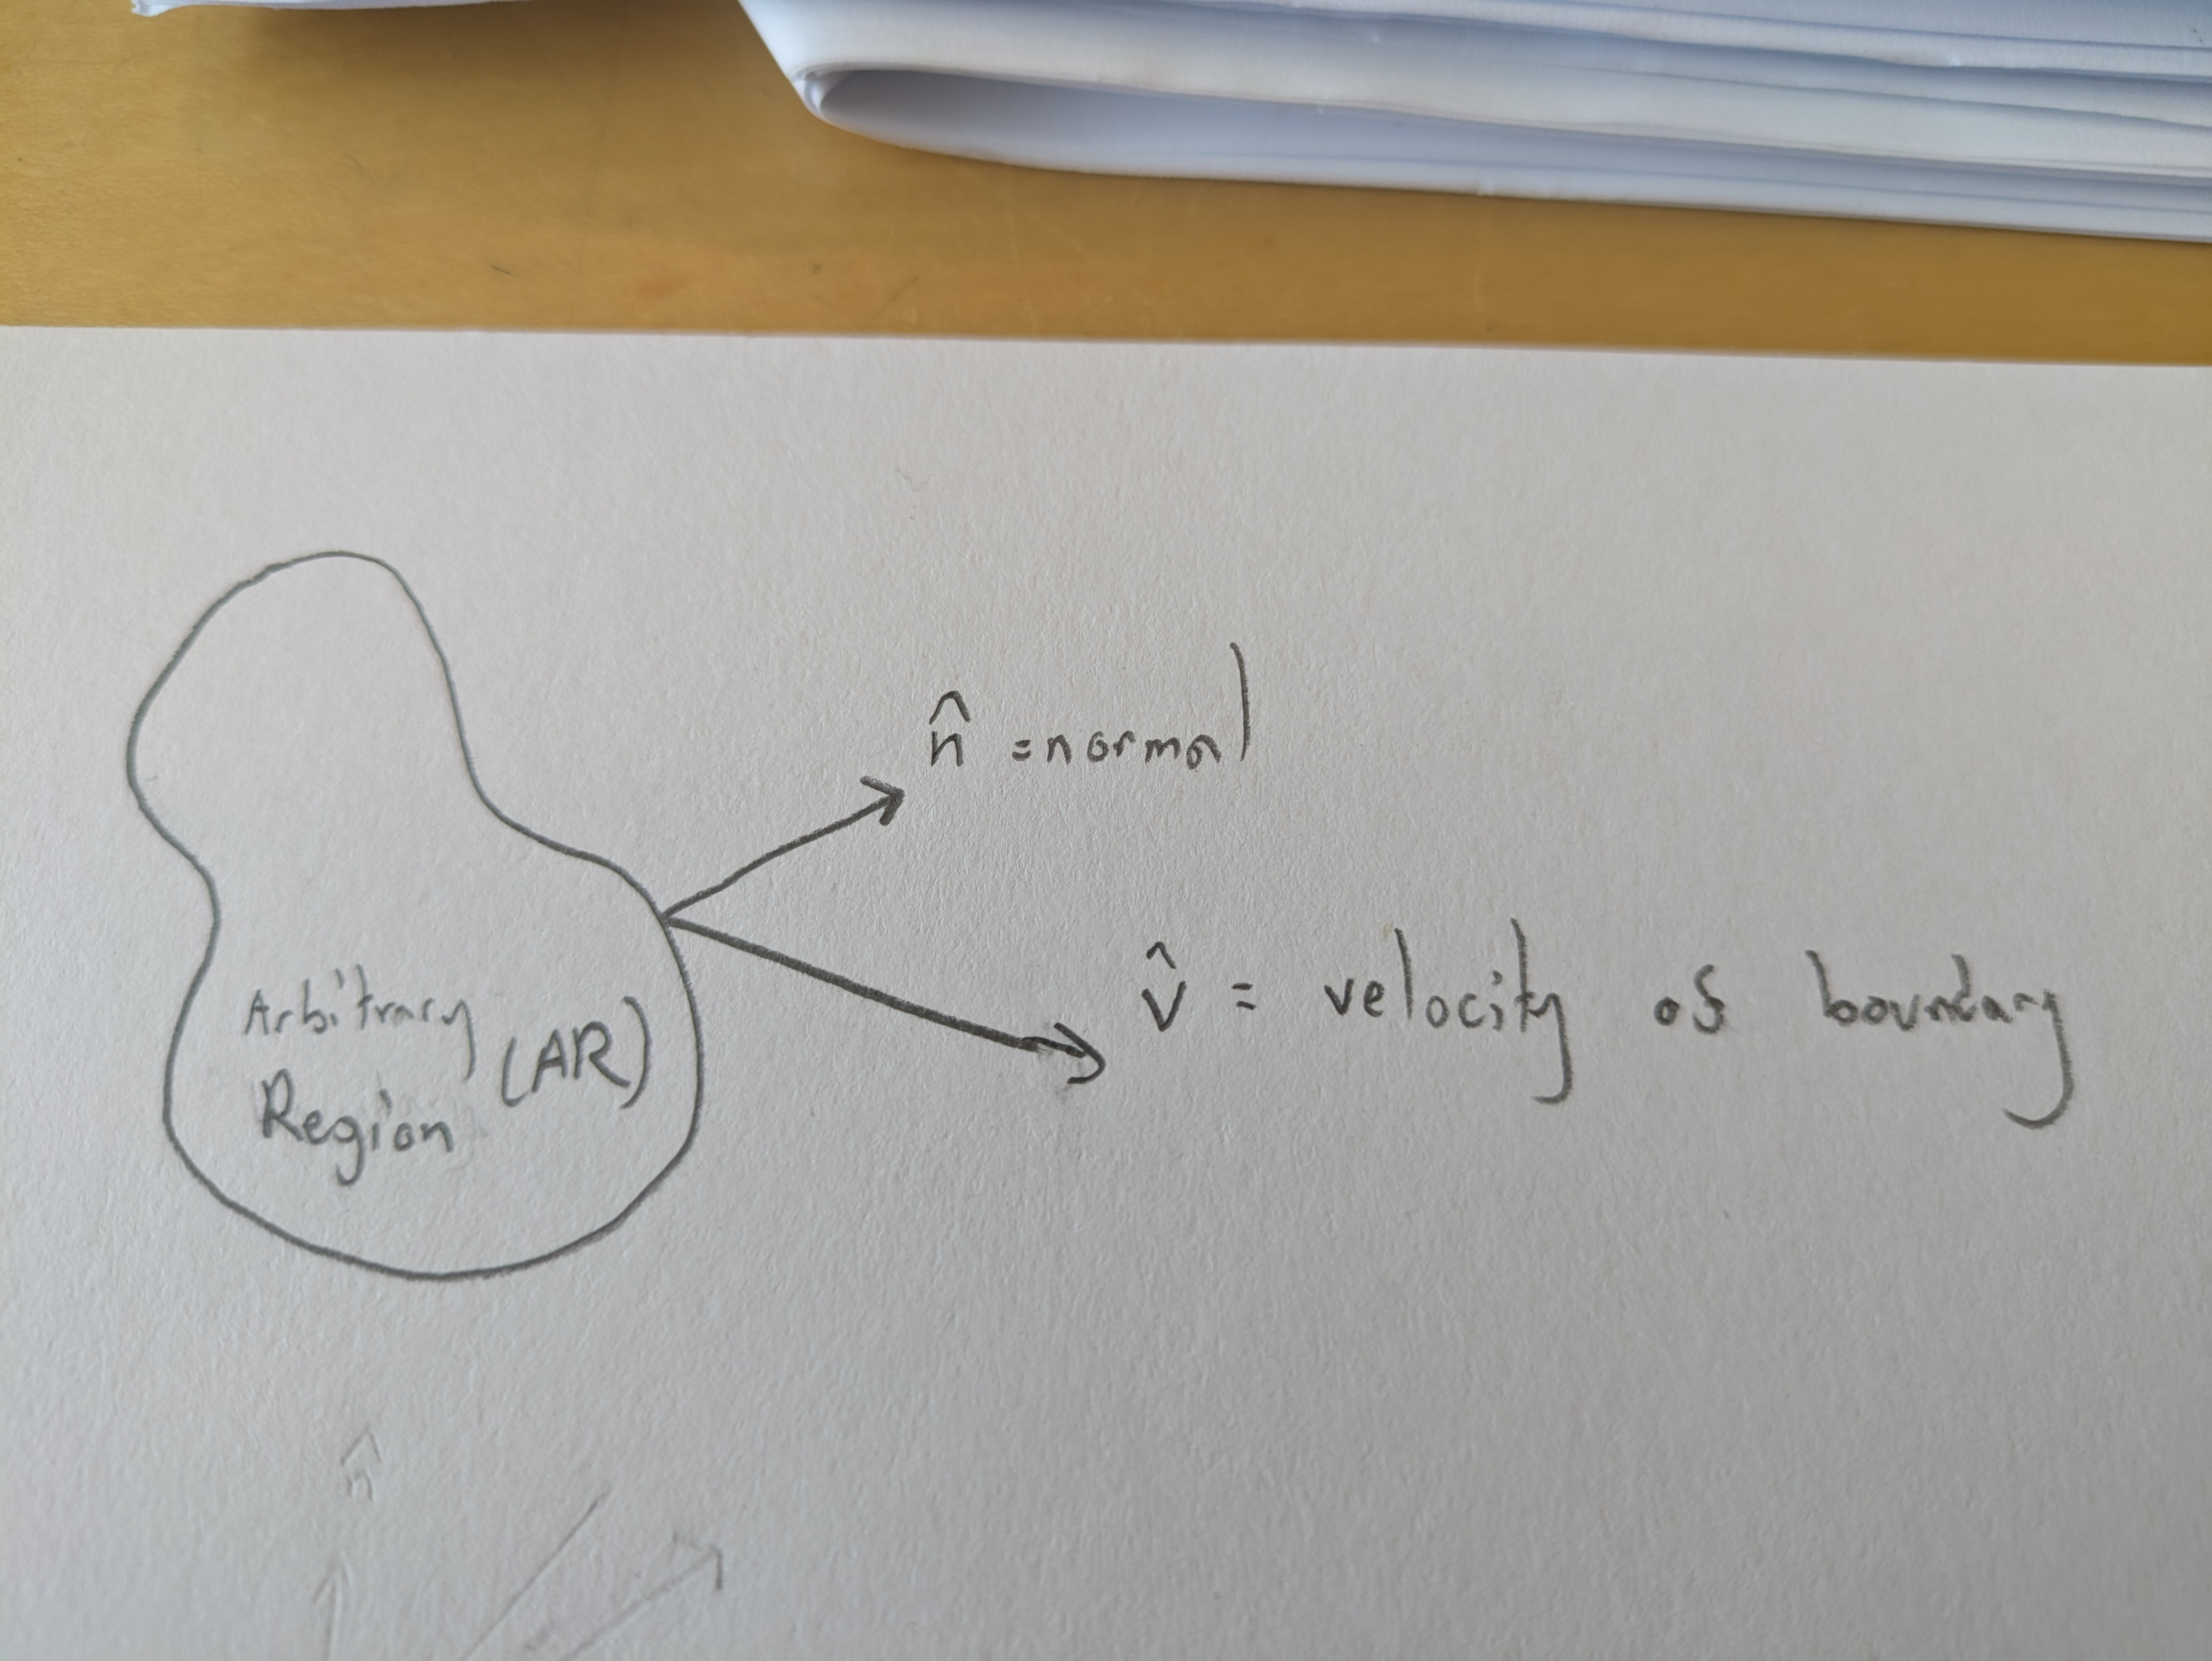
\includegraphics[scale=.07]{moving_boundary.jpg}


\begin{align}
  &\frac{d}{dt}\int_{B_t} \psi dv = \int_{B_t} \pd{\psi}{t}dv + \int_{\partial B_t} \psi u_i da_i
\end{align}

\textcolor{red}{This is confusing, because it is unclear if $u$ is the flow velocity or the boundary velocity, for reynolds transport it is the boundary velocity, but for the derivation in \eqref{eq:transport-theorem} I was under the impression it was the flow velocity $\pd{x}{t}$. It probably applies in both cases, but need to be careful what I am saying.} Renameing the boundary velocity $w$, and plugging in $\psi = \rho$ for mass conservation gives:

\begin{align}
  &\frac{d}{dt}\int_{B_t} \rho dv = \int_{B_t} \pd{\rho}{t}dv + \int_{\partial B_t} \rho w_i n_i ds
\end{align}

Now local conservation of mass can be plugged into the second term on the RHS. This is valid inside the volume, and the second term deals with the moving boundary:

\begin{align}
  &\frac{d}{dt}\int_{B_t} \rho dv = \int_{B_t} -(\rho u_i)_idv + \int_{\partial B_t} \rho w_i n_i ds
\end{align}

and with the divergance theorem:

\begin{align}
  &\frac{d}{dt}\int_{B_t} \rho dv = -\int_{\partial B_t} \rho (u_i - w_i) n_i ds
\end{align}

Now if we think about taking these integrals in a cylinder where the length $L$ goes to zero we can derive the jump condition:

\begin{align}
  &\frac{d}{dt}\int_{B_t} \rho dv = \int_{\text{fluid II}} \rho (u_i - w_i) n_i ds - \int_{\text{fluid I}} \rho (u_i - w_i) n_i ds - \text{curved section integral}
\end{align}

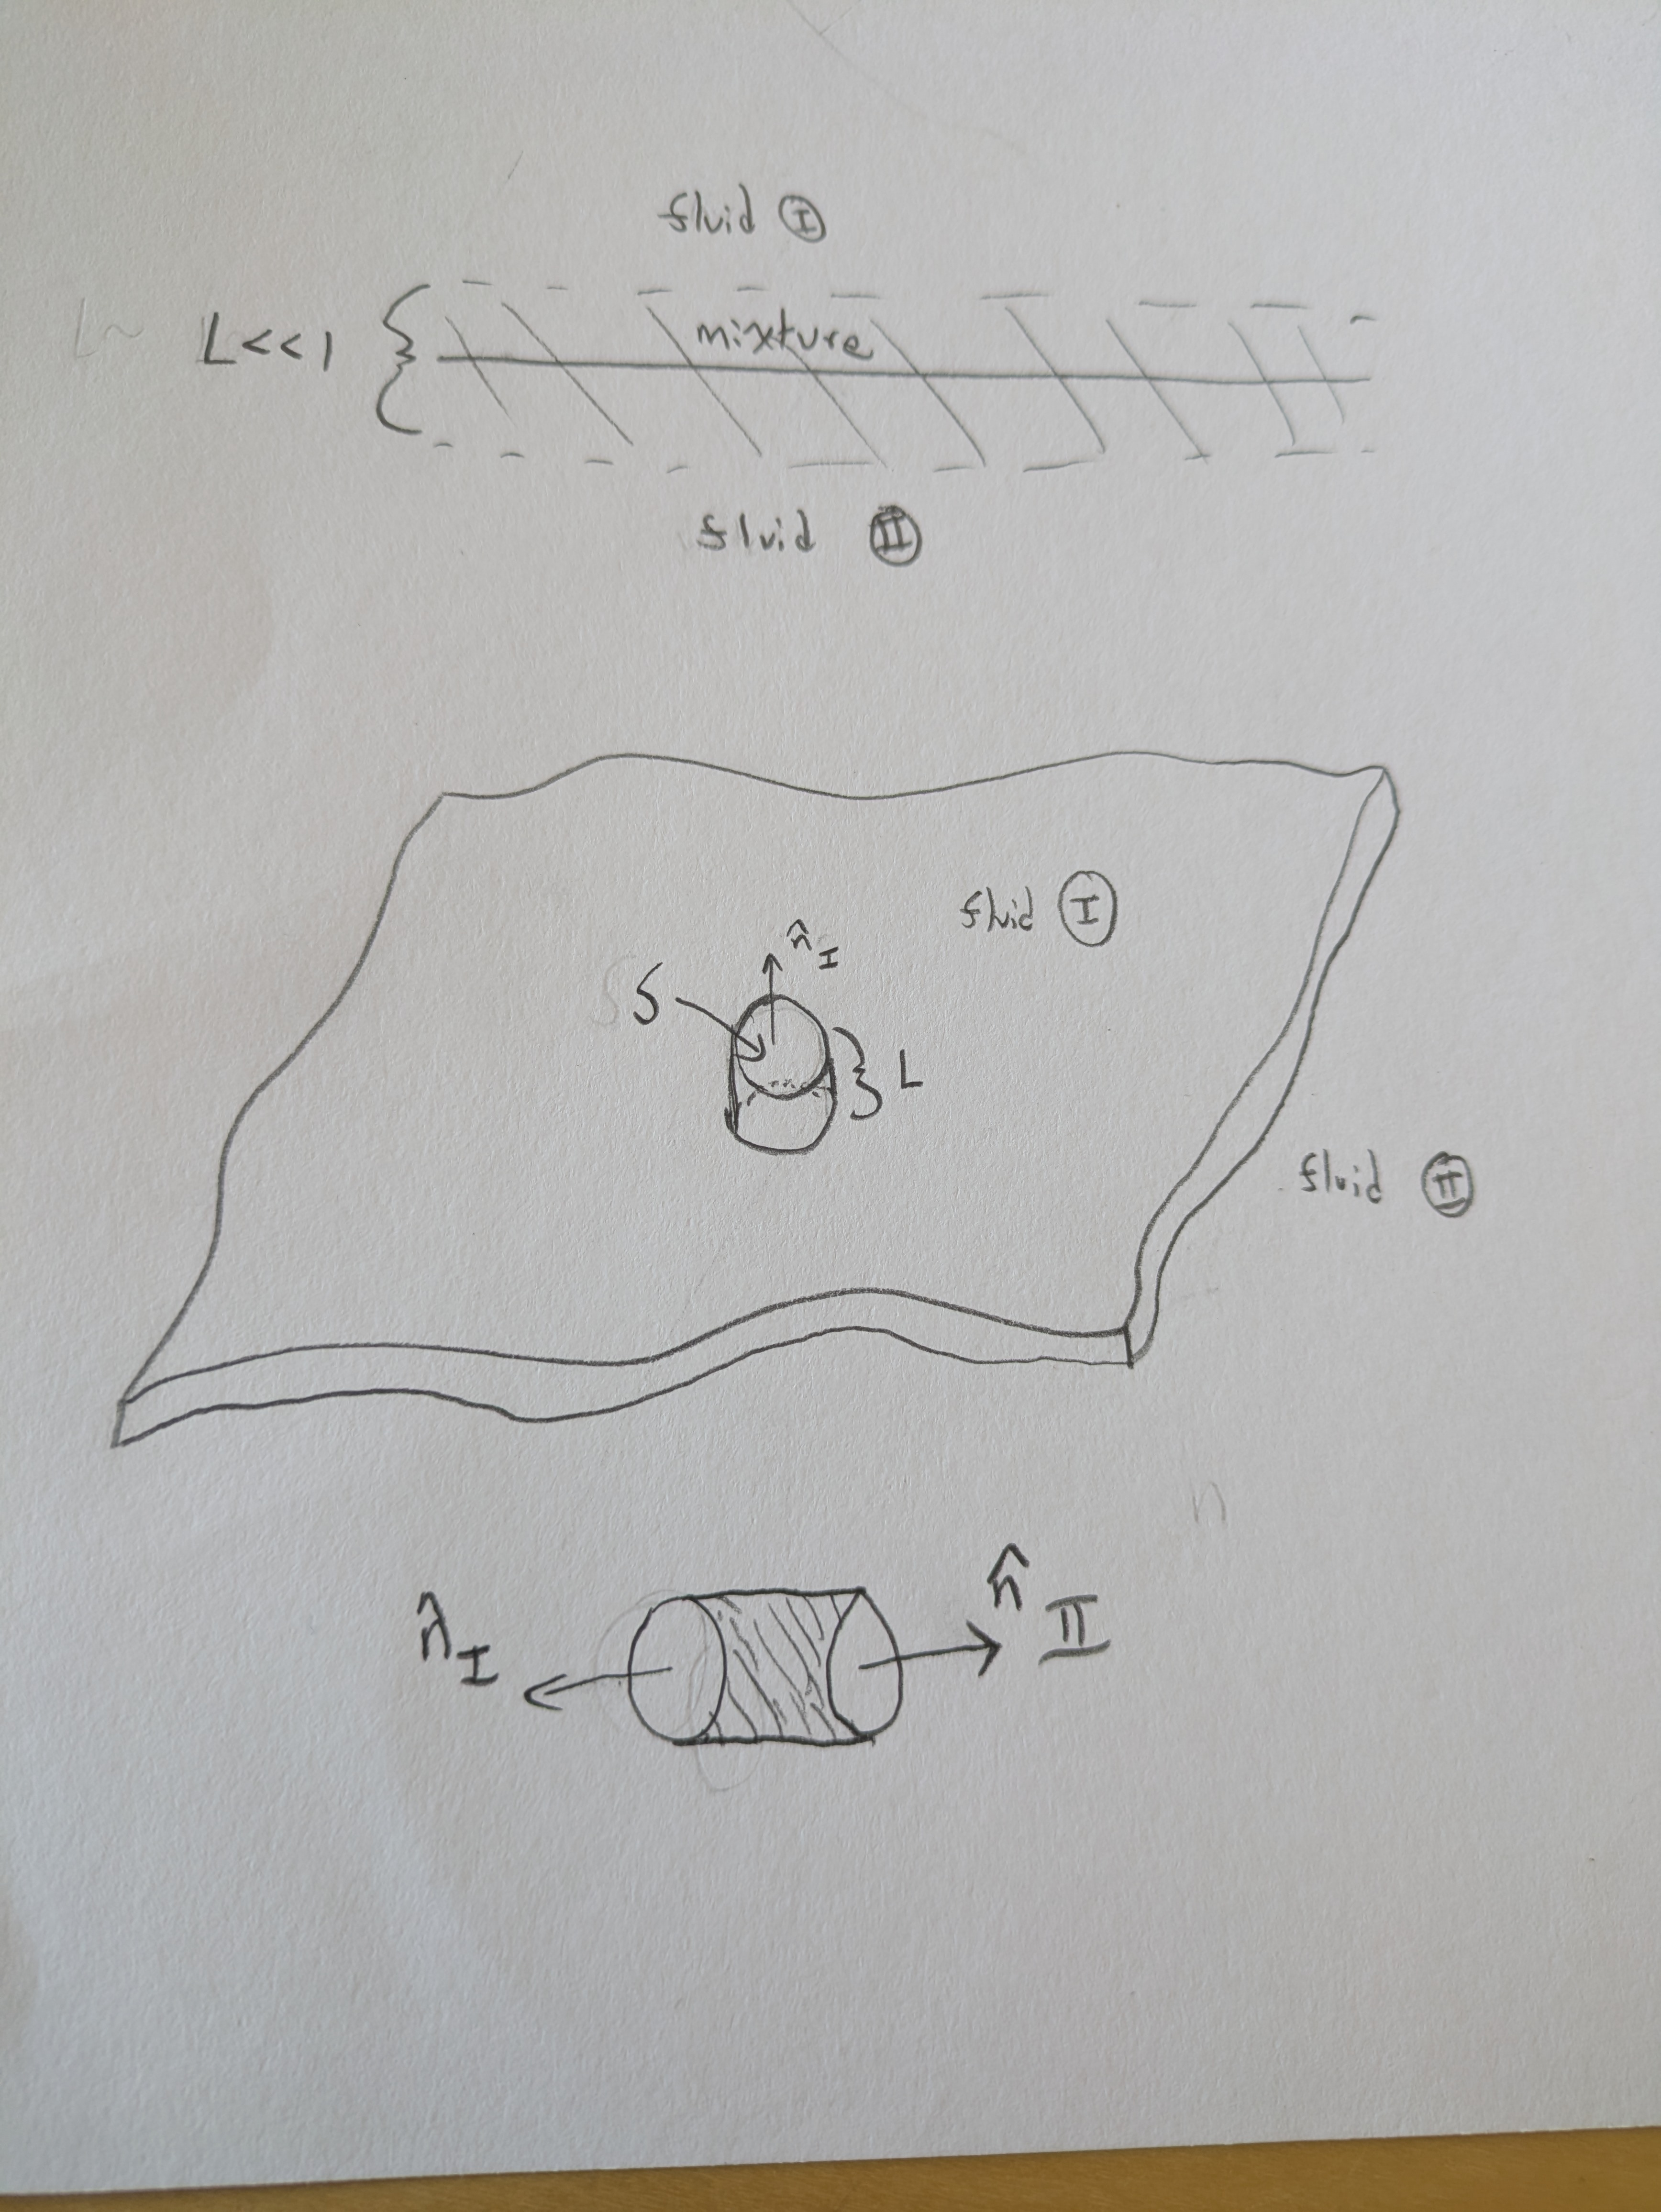
\includegraphics[scale=.1]{fluid_interface.jpg}

The negative sign appears because the normal on one side of the cylinder is the negative of the normal on the other. If we take $L$ to zero the LHS disappears, and the curved part disappears so that:

\begin{align}
  &\int_{\text{fluid II}} \rho (u_i - w_i) n_i ds = \int_{\text{fluid I}} \rho (u_i - w_i) n_i ds
\end{align}

Now shrinking $S$ to a point gives:

\begin{align}
  &[\rho (u_i - w_i) n_i]^+ = [\rho (u_i - w_i) n_i]^-
\end{align}

This condition is esstentially saying that if there is a large density drop the velocity away from the interface must be much higher to conserve mass (assuming $w = 0$).

\subsubsection{momentum conservation}

For momentum conservation the same plugging in of the local equation to reynolds transport theorem gives:

\begin{align}
  &\frac{d}{dt}\int_{B_t} (\rho u_i) dv = \int_{B_t} \pd{(\rho u_i)}{t}dv + \int_{\partial B_t} (\rho u_i) w_j n_j ds\\
  &\frac{d}{dt}\int_{B_t} (\rho u_i) dv = \int_{B_t} \rho F_i + (\sigma_{ij})_j - \int_{B_t} (\rho u_i u_j)_j + \int_{\partial B_t} \rho u_i w_j n_j ds\\
  &\frac{d}{dt}\int_{B_t} (\rho u_i) dv = \int_{B_t} \rho F_i + (\sigma_{ij})_j - \int_{\partial B_t} \rho u_i u_j n_j ds + \int_{\partial B_t} \rho u_i w_j n_j ds\\
  &\frac{d}{dt}\int_{B_t} (\rho u_i) dv = \int_{B_t} \rho F_i + \int_{\partial B_t}\sigma_{ij}n_j ds - \int_{\partial B_t} \rho (u_j - w_j) u_i n_j ds\\
  &\frac{d}{dt}\int_{B_t} (\rho u_i) dv = \int_{B_t} \rho F_i + \int_{\partial B_t}(-pn_i + \tau_{ij}n_j) ds - \int_{\partial B_t} \rho (u_j - w_j) u_i n_j ds \label{eq:momentum-interface-derivation}
\end{align}

Now doing the same integral of the cylinder (and shrinking its length $L$ to zero) the volume integrals disappear:

\begin{align}
  & 0 = 0 - \int_{\text{fluid I}}  \rho (u_i - w_i) u_j n_j ds + \int_{\text{fluid I}}  (-pn_i + \tau_{ij}n_j) ds\\
  &- \int_{\text{fluid II}}  \rho (u_i - w_i) u_j (-n_j) ds + \int_{\text{fluid II}}  (-p(-n_i) + \tau_{ij}(-n_j)) ds
\end{align}

shrinking the surface integrals to a point gives the jump condition:

\begin{align}
  [\rho (u_j - w_j) u_j n_i +  (pn_i - \tau_{ij}n_j)]^+ = [\rho (u_j - w_j) u_j n_i  +  (pn_i - \tau_{ij}n_j)]^-
\end{align}

\textcolor{red}{add physical interpretation.}
  
\section{Schoof and Hewitt Model}

\subsection{Cold}

Cold is the standard:

\begin{align}
  &u_{i,i} = 0 & (\text{incompressiable mass balance})\\
  &\tau_{ij,j} - p_{,i} = \rho g_i & (\text{momentum balance})\\
  &\tau_{ij} = A^{-1/n} D^{1/(n-1)} D_{ij} ~~~ D_{ij} = \frac{1}{2}(u_{i,j} + u_{j,i}) ~~~ D = (D_{ij}D_{ij}/2)^{1/2} & (\text{glen})\\
  & \rho c \left(\pd{T}{t} + u_i T_{,i} \right) - (KT_{,i})_i = a ~~~ a = \tau_{ij}D_{ij} & (\text{energy balance})
\end{align}

\subsection{Temperate}

Now the medium is both ice and water, and is treated as a porous medium with porosity $\phi = \left[\frac{L^3_{fluid}}{L^3_{control}}\right]$, that is always fully saturated. The quantity for conservation of mass is then $\rho^w\phi$, or $\rho^i (1 - \phi) = \left[\frac{m L^3_{fluid}}{L^3_{control}L^3_{fluid}}\right] = \left[\frac{m}{L^3_{control}}\right]$ i.e. total mass of ice or water per control volume. So for the ice mass we get (since $\rho^i = \text{constant}$):

\begin{align}
  \rho^i\pd{(1 - \phi)}{t} + \rho^i [(1 - \phi) u_i]_{,i} = - m \label{eq:conservation-ice-mass}
\end{align}

$m$ is an interal melting rate in $\left[\frac{m}{L^3_{control} t}\right]$. Here we make $u$ the velocity of ice, there is also a water velocity $u^w$ this is in a stationary frame of reference so that $u^w = u + u^l$ where $u^l$ denotes the movement of the water in the ice moving frame of reference. For conservation of water mass we then have:

\begin{align}
  &\rho_w\pd{\phi}{t} + \rho_w[(\phi u + j)_i)]_{,i} = m ~~~ \text{or} ~~~ \rho_w\pd{\phi}{t} + \rho_w[(\phi u^w_i)]_{,i} = m \label{eq:conservation-water-mass}\\
  &j_i = \phi(u_i^w - u_i)
\end{align}


adding conservation of mass and ice togther:

\begin{align}
  &\pd{1}{t} + \pd{\phi}{t} - \pd{\phi}{t} + u_{i,i} - (\phi u_i)_{,i} + (\phi u_i)_{,i} + j_{i,i} = \frac{m}{\rho^w} - \frac{m}{\rho^i}\\
  & u_{i,i} + j_{i,i} = \frac{\rho^w - \rho^i}{\rho^w \rho^i} m \label{eq:conservation-total-mass}
\end{align}


Energy balance can be done in a total, and takes into acount the latent heat of melting. The assumption is made that temperature doesn't change from $T_M$ so there are no temperature gradients or time derivatives, this then gives:

\begin{align}
  mL = a ~~~ \text{or} ~~~ m = \frac{a}{L}
\end{align}

Since its infeasible to solve a momentum balance equation for water velocity, darcy's law is used to find the flux $j$ (\textcolor{red}{appendix of \cite{mckenzie_1984} has a non-empirical derivation of this}):

\begin{align}
  j_i = k_o\phi^\alpha(\rho^wg_i - p^w_{,i}) \label{eq:water-flux}
\end{align}

the water pressure $p^w$ isn't the ice pressure $p^i$ instead it is $p^w + p^e = p^i $, where $p^e$ is the compaction pressure (effective pressure). How to understand this? The total pressure or ice pressure is the water pressure acting inwards?? plus the compaction pressure $p^e$ of ice which is no longer perfectly incompressable. When the ice is compressable then:

\begin{align}
  p^e = \frac{u_{i,i}}{\zeta} ~~~ \zeta = \frac{\eta}{\phi} \label{eq:compaction-relation}
\end{align}

\textcolor{red}{This seems like the units are reversed...}  Where $\zeta$ is bulk viscosity. \cite{mckenzie_1984} scales the bulk viscosity $\zeta \sim \frac{\eta}{\phi}$. As far as I can tell this there is no reason why $\eta$ scales with $\zeta$ instead we are just assuming they are the same, and the inverse scaling with porosity comes from the fact that compaction becomes harder and harder with less pore space which physically/intuatively makes sense.

Given that the compaction pressure is related to the divergence of the ice velocity, conservation of ice mass \eqref{eq:conservation-ice-mass} can be rewritten as:

\begin{align}
  &\rho^i\pd{(1 - \phi)}{t} + \rho^i [(1 - \phi) u_i]_{,i} = - m \\
  &-\pd{\phi}{t} + u_{i,i} - u_i \phi_{,i} - \phi u_{i,i} = -\frac{m}{\rho^i}\\
  &\pd{\phi}{t} + u_i\phi_{,i} = \frac{m}{\rho^i} + (1 - \phi)u_{i,i} ~~~ (\text{using \eqref{eq:compaction-relation}}) \label{eq:ice-mass}\\
  &\pd{\phi}{t} + u_i\phi_{,i} = \frac{m}{\rho^i} - \frac{(1 - \phi)\phi}{\eta}p_e
\end{align}

which is equation 2.15 in \cite{schoof_2016}. Right now we have 3 equations \eqref{eq:conservation-ice-mass}, \eqref{eq:conservation-water-mass}, ande \eqref{eq:conservation-total-mass}, a constitutive law for water flux \eqref{eq:water-flux}, and two unknowns $\phi$, $p$, assuming velocity will be solved for my conservation of mommentum. If we eliminate $p^w$ from \eqref{eq:water-flux} and write it interms of $p$, then it will be easier to see the closed system we are looking for:

\begin{align}
  &j_i = k_0\phi^\alpha(\rho^w g_i + p_{,i}^e - p_{,i})\\
  & j_i = k_0 \phi^\alpha \rho^w g_i + k_0\phi^\alpha p_{,i} - \frac{k_0}{\zeta}\phi^\alpha(u_{j,j})_{,i}
\end{align}

plugging this into \eqref{eq:conservation-total-mass} gives:

\begin{align}
  & u_{i,i} + k_0\rho^w\partial_i(\phi^\alpha g_i) + k_0 \partial_i (\phi^\alpha \partial_i p) - \frac{k_0}{\zeta}\partial_i\left(\phi^{\alpha} \partial_i\partial_ju_{j}\right) = \frac{\rho^w - \rho^i}{\rho^w \rho^i} m \\\label{eq:total-mass-velocity}
  & u_{i,i} + k_0\rho^w\partial_i\phi^\alpha g_i - \frac{k_0}{\zeta}(\partial_i\phi^{\alpha} \partial_i(\partial_ju_{j}) + \phi^{\alpha} \partial_i\partial_i\partial_ju_{j}) + k_0 (\partial_i\phi^\alpha \partial_i p + \phi^\alpha \partial_i\partial_i p)= \frac{\rho^w - \rho^i}{\rho^w \rho^i} m \\\label{eq:total-mass-velocity}
\end{align}

which is an equation purely interms of $p$, $u$ and $\rho$. (Alternatively darcy's law could have been plugged into \eqref{eq:conservation-water-mass} and this would have also closed the system.) Given a velocity from momentum conservation $\phi$ can be solved for using \eqref{eq:ice-mass}, and $p$ can be solved for using \eqref{eq:total-mass-velocity}.

Putting these equations all in the same place (and writing them in vector notation:

\begin{align}
  &\pd{\phi}{t} + u \cdot \nabla \phi = \frac{m}{\rho^i} + (1 - \phi)(\nabla \cdot u) ~~~ (\text{conservation of ice mass: solve } \phi)\\ \label{eq:conservation-ice-mass-2}
  &\nabla \cdot u + k_0\rho^wg\pd{(\phi^{\alpha})}{x_3} - \frac{k_0}{\zeta}(\nabla \phi^\alpha\nabla(\nabla \cdot u) + \phi^\alpha \nabla^2(\nabla \cdot u)) + k_0(\nabla \phi^\alpha\nabla p + k_0\phi^\alpha \nabla^2 p)\\ \label{eq:overall-mass-conservation} \nonumber
  &\ = \frac{\rho^w - \rho^i}{\rho^w \rho^i} m ~~~ (\text{overall mass conservation: solve } p)\\ 
  & \nabla \cdot ((1-\phi)\tau) - \nabla \left[p - \frac{\phi^2}{\eta}\nabla \cdot u\right] = -(1 - \phi) \rho g - \phi \rho_w g ~~~ (\text{conservation of momentum: solve } u)\\ \label{eq:conservation-of-momentum-temperate}
  &\tau_{ij} = A D^{1/n-1}(D_{ij} - \frac{1}{3}D_{kk}\delta_{ij}) ~~~ (\text{glen's flow law with pressure removed})
\end{align}

A few conceptual things to remember:


\begin{outline}
\1 The mixture is not compressable in the sense that $p^i$ or $p^w$ are constant. It is compressable in the sense the divergance of ice velocity doesn't have to be zero as it moves into or out of the pore space. We have replaced an equation state like $\rho(p,T)$ with $p(\nabla \cdot u)$.
\1 how is $m$ determinated? From conservation of energy we got $m = \frac{a}{L}$, where $a=\tau_{ij}D_{ij}$, and $L$ is the latent heat of melting. This is another way that momentum is coupled to the two mass conservations laws. Essentially melts forces the porosity equation.
\1 Can we give a physical description of each term? For \eqref{eq:conservation-ice-mass-2}:

\2 $\pd{\phi}{t}$ is the time rate of change of porosity at a fixed point.
\2 $u \cdot \nabla \phi$ is the avection of porosity with a moving solid ice matrix.
\2 $\frac{m}{\rho^i}$ is a conversion of melt to fully water saturated pore space.
\2 $(1 - \phi)(\nabla \cdot u)$ is the compaction and dilation of the ice matrix. That is, if $\nabla \cdot u > 0$ then the ice matrix is expanding, giving rise to a positive increase in pore space, the opposite is true if $\nabla \cdot u < 0$.

\1 For \eqref{eq:overall-mass-conservation}:

\2 $\nabla \cdot u$ is the local divergence or compaction.

\2 $k_0\rho^wg\pd{\phi^\alpha}{x_3}$ is a buoyancy term that drives darcy flow, so that if porosity increases with height flow wants to be upward. Then, $g \pd{(\phi^\alpha)}{x_3} < 0$ meaning that fluid is converging on that point, and therefore to balance, the ice must be diverging $\nabla \cdot u > 0$, and inversely if porosity is decreasing with fluid diverging, and ice is converging.

\2 $\frac{k_0}{\zeta}(\nabla \phi^\alpha\nabla(\nabla \cdot u))$ with units of $\frac{m^2}{Pa s} \frac{kg}{ms}\frac{1}{m^2s} = \frac{1}{s}$ which matches up with $\nabla \cdot u$. This is an interaction between compaction gradients, and porosity gradients. If we imagine there is an increase in ice matrix dilation so that $\nabla(\nabla \cdot u) > 0$, and there is also there is a positive porosity gradient $\nabla \phi > 0$, these together make this term large and positive representing...\textcolor{red}{This is confusing me...}

\2 $\phi^\alpha \nabla^2(\nabla \cdot u)$ This is the laplacian of compaction. If we imagine we are at a point where compaction is the highest and lower all around us i.e. ice is maximally diverging, then this term is highly negative and could be balanced with lots of melt on the RHS for instance? \textcolor{red}{finish this...}

\1 For \eqref{eq:conservation-of-momentum-temperate}:

\2 $\nabla \cdot ((1-\phi)\tau)$ This is just friction, but scaled by the ice matrix fraction and neglecting frictional forces of the water.

\2 $\nabla p$ This the pressure gradient term for the ice

\2 $\nabla(\frac{\phi^2}{\eta}\nabla \cdot u)$ with units $\frac{1}{m}\frac{kg}{ms}frac{1}{s} = \frac{kg}{m^2 s^2}$ which lines up with $\nabla \cdot \tau$. This is saying the gradient of compaction is generating a force. Would like more physical intuition for this.

\end{outline}

\subsection{Interface conditions}

Applying the jump conditions derived earlier, conservation of mass is split between ice and water:

\begin{align}
  [\rho^I(1 - \phi)(u_i - w_i) + \rho^w \phi (u_i - v_i) + \rho^w j_i]n_i = \rho(u_i - v_i)n_i
\end{align}

\textcolor{red}{Why is the darcy flux not scaled by the velocities?}
$\rho(u_i - v_i)n_i$ is the mass flux across the interface.
For the momentum interface conditions looking at the derivation of \eqref{eq:momentum-interface-derivation}, the last term will be zeroed out because interial terms in stokes flow are 0. This leaves us with:

\begin{align}
  [(pn_i - \tau_{ij}n_j)]^+ = [(pn_i - \tau_{ij}n_j)]^-
\end{align}

\textcolor{red}{it looks like there is a typo in schoof  hewitt, and $n_j$ shouldn't appear twice in the temperate fricition term.} Splitting this again between water and ice gives (up to a sign convention):

\begin{align}
    [-\phi p^w\delta_{ij} n_j - (1 - \phi)p\delta_{ij}n_j + (1 - \phi)\tau_{ij}n_j]^+ = [(p\delta_{ij}n_j - \tau_{ij}n_j)]^-
\end{align}

The temperature at the interface is set to the melting point $T_m$, and the velocities are set to be the same. Lastly as a sort of ``conservation of energy'' interface conditions there is the stephan condition which says:

\begin{align}
  [\rho^wL\phi(u_i-w_i) + \rho^wLj_i - KT_{,i}]^+ n_i = -KT_{,i}^- n_i
\end{align}

This is saying that the latent heat at the boundary is equal to the flux discontinuity. In the one-phase problem meaning the case were in the temperate ice $T=T_m$ there is no $T_{,i}^+$ so that term disapears. This interface condition can be derived from a similar cylinder argument as the other interface conditions. \cite{Andreucci}

\subsection{non-dimensionalization and scaling}

So far we gave the equations from \cite{schoof_2016}, fully plugged in so that there are 5 equations for 5 unknowns. Using there scaling I redo the non-dimensionalization. They take non-dimensional variables:

\begin{align*}
  & x = [x]x^*, ~~~ u = [u]u^*, ~~~ t = [x]/[u]t^* ~~~ a = [a]a^*, ~~~ T = T_{ref} + \frac{[a][x]^2}{K}T^*, ~~~ \phi = \frac{\rho c [T]}{\rho^w L}\phi^*, ~~~ j = \frac{[a][x]}{\rho^w L}j^*\\
  & p^e = \frac{[\eta][a]}{\epsilon\rho^wL}p^{*e}, ~~~ p^r = \frac{[\eta][u]}{[x]}p^{*r}
\end{align*}
  
\textcolor{red}{Only one that doesn't seem completely intuative is reduced pressure}. Where $\epsilon = \frac{\rho c [T]}{\rho^w L}$. First doing conservation of momentum:

\begin{align*}
  & \frac{1}{[x]}\nabla^* \cdot ((1-\epsilon\phi^*)\tau) - \nabla p + \nabla\left[\frac{\phi^2}{\eta}\nabla \cdot u\right] = -(1 - \phi) \rho g - \phi \rho_w g\\
  & \frac{1}{[x]}\nabla^* \cdot ((1-\epsilon\phi^*)\tau) - \nabla p + \rho g + \nabla\left[\frac{\phi^2}{\eta}\nabla \cdot u\right] = \phi\rho g - \phi \rho_w g\\
  & \frac{1}{[x]}\nabla^* \cdot ((1-\epsilon\phi^*)\tau) - \nabla p_r + \nabla\left[\frac{\phi^2}{\eta}\nabla \cdot u\right] = \phi\rho g - \phi \rho_w g\\
  & \frac{1}{[x]}\nabla^* \cdot ((1-\epsilon\phi^*)\tau) - \frac{1}{[x]}\frac{[\eta][u]}{[x]}\nabla^* p^*_r + \frac{1}{[x]}\nabla^*\left[\epsilon\frac{[\eta][a]}{\epsilon \rho^w L}\phi^*p_e^*\right] = \epsilon \phi^* g (\rho - \rho^w)\\
  & \tau_{ij} = A^*D^{1/n-1}\left(D_{ij} - \frac{1}{3}D_{kk}\delta_{ij}\right)
\end{align*}

\subsection{1D polythermal: Schoof hewitt}

The scaled equations become for temperate ice:

\begin{align*}
  &\nabla \cdot (k \phi^\alpha( g + \delta \nabla p_e) = \frac{\phi p_e}{\eta} \\
  & Pe \left(\pd{\phi}{t} + u \cdot \nabla \phi \right) + \frac{\phi p_e}{\eta}  = a
\end{align*}

and for cold ice:

\begin{align*}
  & Pe \left(\pd{T}{t} + u \cdot \nabla T\right)  - \nabla^2 T = a
\end{align*}

first we reduce these to 1D and then consider boundary conditions.

For the temperate ice:

\begin{align*}
  &\nabla \cdot (\kappa \phi^\alpha( g + \delta \nabla p_e)) = \frac{\phi p_e}{\eta} \rightarrow \nabla \cdot (\kappa \phi^\alpha g + \kappa\phi^\alpha\delta \nabla p_e) = \frac{\phi p_e}{\eta}\\
  &\pd{}{z}\kappa \phi^\alpha g + \pd{}{z}\left(\kappa\phi^\alpha\delta\pd{}{z}p_e\right) = \frac{\phi p_e}{\eta}\\
  & Pe \left(\pd{\phi}{t} + u \cdot \nabla \phi \right) + \frac{\phi p_e}{\eta}  = a \rightarrow Pe\pd{\phi}{t} + Pe u \pd{\phi}{z} + \phi p_e = a
\end{align*}

So the coupled system is:

\begin{align*}
  &\pd{}{z}\kappa \phi^\alpha g + \pd{}{z}\left(\kappa\phi^\alpha\delta\pd{}{z}p_e\right) = \frac{\phi p_e}{\eta}\\
  &Pe\pd{\phi}{t} + Pe u \pd{\phi}{z} + \phi p_e = a
\end{align*}

Assuming the temperate region is below the the cold region, and ice motion is downwards, the boundary conditions are:

\begin{align*}
  T(H) = T_0\\
  T(0) = T_m\\
  p_e(0) = N_0\\
\end{align*}

At the interface we have:

\begin{align*}
  -\pd{T}{z} = 0\\
  \phi = 0\\
  \kappa \phi^\alpha( g + \delta \nabla p_e) = 0
\end{align*}

For the cold region we solve:

\begin{align}
  Pe\pd{T}{t} + Pe u \pd{T}{z} - \pdt{T}{z} = a \\
  T(H) = T_0\\
  \pd{T(\Gamma)}{z} = T(\Gamma) = 0
\end{align}

For the temperate ice we solve for $p_e$, and $\phi$:

\begin{align}
  &\pd{}{z}\left(\kappa\phi^\alpha\left(g + \delta\pd{}{z}p_e\right)\right) = \frac{\phi p_e}{\eta} \label{eq:pe-equation}\\
  &p_e(0) = N_0\\
  &\left(\kappa \phi^\alpha\left( g + \delta \pd{}{z} p_e\right)\right)\bigg\rvert_{z=\Gamma} = 0 ~~~ \text{or} ~~~ p_e(\Gamma) = 0\\
\end{align}
\begin{align}
  &Pe\pd{\phi}{t} + Pe u \pd{\phi}{z} + \phi p_e = a \label{eq:phi-equation}\\
  &\phi(\Gamma) = 0\\
\end{align}

\subsubsection{normal finite element}

Cold region:

\begin{align*}
  &\int_{\Omega_T} \psi_i\pd{T}{t} + \int_{\Omega_T} u \pd{T}{z}\psi_i dz - \frac{1}{Pe}\int_{\Omega_T} \pdt{T}{z}\psi_i dz = \int_{\Omega_T} a\psi_i dz ~~~ \forall i \\
  &\int_{\Omega_T} \psi_i\pd{T}{t} + \int_{\Omega_T} u \pd{T}{z}\psi_i dz + \frac{1}{Pe}\int_{\Omega_T} \pd{T}{z}\pd{\psi_i}{z} dz - \pd{T}{z} \psi_i \bigg\rvert_0^L = \int_{\Omega_T} a\psi_i dz ~~~ \forall i \\
  & M\pd{T}{t} + uST + \frac{1}{Pe}KT = \frac{1}{Pe}F
\end{align*}

Where:

\begin{align*}
  M_{ij} = \int_k\psi_i\psi_j ~~~ S_{ij} = \int_k\psi_i\pd{\psi_j}{z} ~~~ K_{ij} = \int_k\pd{\psi_i}{z}\pd{\psi_j}{z} ~~~ F_i = \int_ka\psi_i
\end{align*}


Doing Crank-Nicolson in time (could make the advective part explict in the future) gives:

\begin{align*}
  & M\frac{T^{n+1} - T^n}{\Delta t}   = \frac{1}{2}\left(\frac{1}{Pe}F^{n+1} - uST^{n+1} - \frac{1}{Pe}KT^{n+1} +\frac{1}{Pe}F^n - uST^n - \frac{1}{Pe}KT^n\right) = \\
  & \left(M + \frac{\Delta t}{2}\left(uS + \frac{1}{Pe}K\right)\right)T^{n+1} = \left(M - \frac{\Delta t}{2}\left(uS + \frac{1}{Pe}K\right)\right)T^{n} + \frac{F^{n+1} + F^n}{2}
\end{align*}

For the temperate region solve \eqref{eq:pe-equation} with previous $\phi$ for $P_e$ then use to solve \eqref{eq:phi-equation}:

\begin{align*}
  &\pd{}{z}\left(\kappa\phi^\alpha\left(g + \delta\pd{}{z}p_e\right)\right) = \frac{\phi p_e}{\eta}\\
  &\int_{\Omega_T}\left(\pd{}{z}\left(\kappa\phi^\alpha\left(g + \delta\pd{p_e}{z}\right)\right)\right) \psi_i dz = \int_{\Omega_T}\frac{\phi p_e}{\eta}\psi_idz\\
  &-\int_{\Omega_T}\left(\kappa\phi^\alpha\left(g + \delta\pd{p_e}{z}\right)\right) \pd{\psi_i}{z} dz + \left(\kappa\phi^\alpha\left(g + \delta\pd{p_e}{z}\right)\right)\psi_i \bigg\rvert_R^L= \int_{\Omega_T}\frac{\phi p_e}{\eta}\psi_idz\\
  &-\int_{\Omega_T} \kappa\phi^\alpha g \pd{\psi_i}{z}dz -\int_{\Omega_T} \kappa\phi^\alpha\delta\pd{p_e}{z}\pd{\psi_i}{z}  dz + \left(\kappa\phi^\alpha\left(g + \delta\pd{p_e}{z}\right)\right)\psi_i \bigg\rvert_R^L= \int_{\Omega_T}\frac{\phi p_e}{\eta}\psi_idz\\
  &-\kappa \delta K p_e - \frac{1}{\eta}M p_e = \kappa g F_g - \left(\kappa\phi^\alpha\left(g + \delta\pd{p_e}{z}\right)\right)\psi_i \bigg\rvert_R^L\\
  & K_{ij} = \int_k\pd{\psi_i}{z}\phi^{\alpha}\pd{\psi_i}{z} ~~~ M_{ij} = \int_k \psi_i \phi \psi_j ~~~ F_i = \int_k \phi^{\alpha}\pd{\psi_i}{z}
\end{align*}

Finally the porosity equation is:




\subsection{1D polythermal model: Haseloff}

Here we follow \cite{haseloff_2019} here, and take a cross section of an ice stream with ridges on either side, with $x$ as the downstream flow direction, $y$ the across stream direction, and $z$ verticle. We assume that velocities $u$ occur only in the downstream direction $x$, and are not dependent on $x$. The geometry of the stream is assumed to be flat of height $H$, while the ridges follow the typical SIA profile \cite{Greve_2009}:

\begin{align*}
  -\frac{2}{n+2}(\rho g)^n \pd{}{y}\left(\bar{A} H^{n+2}\left|\pd{(H + z_b)}{y}\right|^{n-1}\pd{(H+z_b)}{y} = \dot{a}\right)
\end{align*}

where $z_b$ is the bed elevation. This is a boundary value ODE problem with boundary conditions:

\begin{align*}
  &H + z_b ~~~~ \text{at the stream}\\
  &\pd{(H + z_b)}{y} = 0 ~~~ \text{at the top of the ridge/edge of domain}
\end{align*}

velocity is 1D and invarient execept in the $y$ direction, so that momentum balance is:

\begin{align*}
  &\pd{}{y}\left(\eta H\pd{u}{y}\right) - \tau_b = -\rho g H \sin \alpha ~~~ \text{in the stream}\\
  &u = 0 ~~~ \text{in the ridge}
  \end{align*}

  where $\alpha$ is the downstream slope. where in the middle of the stream there is no variation in $y$ so $\pd{u}{y} = 0$, and at the far end of the ridge $u = 0$. \textcolor{red}{Given this solution we zero out the rest of $u$ once it becomes zero in the ridge???}
  In the cold ice domain conservation of energy is with temperature:

\begin{align*}
  -k\pdt{T}{z} = \frac{\overline{A^{-1/n}}}{2^{1/n}}\left|\pd{u}{y}\right|^{1+n/n}
\end{align*}

Where the lhs is the expression for heat dissipation. This has a dirichlet condition on the surface, and then interface conditions if the temperate region reaches above the bed, and dirchlete conditions if its still on the bed.




\subsection{2D polythermal model}

\section{Aschwanden Model}

\section{Hutter Textbook Model}

%In \cite{hutter_theoretical_1983} there is a model of a polythermal glaicer, here is a summary of that model:





\bibliography{refs}{}
\bibliographystyle{apalike}

\end{document}
